\documentclass{beamer}
%\usetheme{Rochester}
\usetheme{Copenhagen}
%\usetheme{Madrid}
\usepackage{graphicx}

\title{The Go Programming Language}
\subtitle{http://www.golang.org \\ CS 239: Parallel Programming Languages}
\author{Raghu Prabhakar \\ Rohit Kumar}
\newcommand{\bigsize}[1]{\color{red}{\fontsize{60}{60}{\textbf{\selectfont #1}}}}
\newcommand{\medsize}[1]{\fontsize{25}{25}\selectfont #1}
\date{June 2, 2011}
\begin{document}

\begin{frame}
\begin{center}

\includegraphics[width=1in]{gopher.png}
\end{center}
\titlepage
\end{frame}

\begin{frame} {About Go}
\begin{itemize}
  \item Developed by Google. Released in 2009.
  \item Rob Pike, Ken Thompson, Robert Griesemer
  \item Compiled, garbage collected, concurrent, statically typed,
    imperative. 
  \item UTF-8 Support
  \item Borrows from CSP, Occam and Erlang
  \item Compilers: 6g, 8g, gcc 
\end{itemize}
\end{frame}

\begin{frame}[fragile]
\frametitle{Basics}
    {\small
\begin{verbatim}
package main;
import ( "fmt" );
const N = 256;
func addArray(a []int) int {
  var sum int = 0
  for i:= 0 ; i< len(a); i++ {
    sum += a[i]
  }
  return sum;
}
func main() {
  var a []int; a = make([]int,N);
  for i:= 0; i<N; i++ {
    a[i] =  i %10; 
  }
  sum := addArray(a)
  fmt.Println(sum) 
}		
\end{verbatim}
}
\end{frame}

\begin{frame}[fragile]
\frametitle{Concurrency}
  \begin{itemize}
    \item Go statement -- spawn threads
    \item Channels -- send and receive messages
    \item Others -- WaitGroup, do.Once, etc    
  \end{itemize}
\end{frame}

\begin{frame} [fragile]
\frametitle{Go-routines}
\begin{itemize}
  \item Call \verb=runtime.GOMAXPROCS(n)= to run on multiple processors
  \item \verb=go= statement $\approx$ \verb=async= in X10
\end{itemize}
\begin{center}
\begin{verbatim}
                go mapblock(start, end)
\end{verbatim}
\end{center}
\begin{itemize}
\item Starts function \verb=mapblock= in a new thread with arguments \verb=start= and \verb=end=
\item \verb=mapblock= is called a go-routine
\end{itemize}

\end{frame}

\begin{frame} [fragile]
\frametitle{Channels}
\begin{itemize}
\item Used to send and receive messages
\item Channels are typed
\end{itemize}
\begin{verbatim}
        var ch = make(chan int) 
        ch <- 42 // send 
        var i = <- ch // receive        
\end{verbatim}
\begin{center}
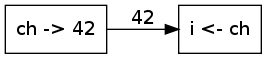
\includegraphics[width=2in]{channel.png}
\end{center}
\end{frame}

\begin{frame}{Channels}

\begin{itemize}
\item Buffered and unbuffered
\item Unbuffered -- block on send and receive
\item Buffered  -- block on send only if buffer is full. Block on receive.

\end{itemize}
\end{frame}

\begin{frame}[fragile]
\frametitle{Channels}
\begin{itemize}
\item Channels can be used to model X10's \verb=finish= statement
\end{itemize}
\begin{verbatim}
        var ch = make(chan bool)
        for i:=0; i < n ; i++ {
                go func() { 
                        // do something
                        ch <- true
                } ()
        }
\end{verbatim}
\pause
\begin{verbatim}
        // drain the channel
        for i:=0; i < n; i++ {
                <- ch
        }
        close(ch)
        
\end{verbatim}
\end{frame}


\begin{frame} [fragile]
\frametitle{WaitGroup}
\begin{itemize}
\item A better construct to model X10's \verb=finish= statement
\end{itemize}
\begin{verbatim}
        var wg sync.WaitGroup
        for i:=0; i < n ; i++ {
                wg.Add(1)
                go func() { 
                        // do something
                        wg.Done()
                } ()                
        }
        wg.Wait() // wait for all go-routines to finish
\end{verbatim}


\end{frame}

\begin{frame}[fragile] 
\frametitle{Map Reduce}
\begin{itemize}
  \item Sequential
  \item $\frac{n}{k}$ version of map reduce using arrays
  \item Streaming map reduce using channels
\end{itemize}
\end{frame}

\begin{frame} {Parallel Prefix Sum}
\end{frame}

\begin{frame} [fragile]
\frametitle{Other Things}
\begin{itemize}
\item The \verb=select= statement
\item sync.Once.Do
\item Locks and mutexes
\item More in the \verb=sync= package
\end{itemize}
\end{frame}

\end{document}
